\documentclass[11pt,a4paper]{article}

% ── Packages ──────────────────────────────────────────────────
\usepackage[margin=2cm]{geometry}
\usepackage{amsmath,amssymb,amsthm}
\usepackage[most]{tcolorbox}
\usepackage{graphicx}
\usepackage{enumitem}
\usepackage{booktabs}
\usepackage{tikz}
\usetikzlibrary{arrows.meta,positioning,calc}
\usepackage{hyperref}
\hypersetup{colorlinks=true,linkcolor=blue!70!black,urlcolor=blue!50!black}

% ── Theorem-like environments ─────────────────────────────────
\theoremstyle{definition}
\newtheorem{definition}{Definition}[section]
\newtheorem{example}{Example}[section]
\theoremstyle{plain}
\newtheorem{theorem}{Theorem}[section]
\newtheorem{property}{Property}[section]

% ── tcolorbox styles ──────────────────────────────────────────
\newtcolorbox{keytakeaways}{
  colback=blue!5!white,
  colframe=blue!60!black,
  fonttitle=\bfseries,
  title={Key Takeaways},
  sharp corners,
  boxrule=0.8pt
}

\newtcolorbox{warning}{
  colback=red!5!white,
  colframe=red!70!black,
  fonttitle=\bfseries,
  title={Common Pitfall / Warning},
  sharp corners,
  boxrule=0.8pt
}

\newtcolorbox{remark}{
  colback=yellow!5!white,
  colframe=orange!70!black,
  fonttitle=\bfseries,
  title={Important Remark},
  sharp corners,
  boxrule=0.8pt
}

\newtcolorbox{formulabox}[1][]{
  colback=green!3!white,
  colframe=green!50!black,
  fonttitle=\bfseries,
  title={#1},
  sharp corners,
  boxrule=0.8pt
}

% ── Document ──────────────────────────────────────────────────
\begin{document}

\begin{center}
{\LARGE\bfseries Project Management -- Part 3}\\[6pt]
{\large Revision Sheet}\\[4pt]
{\small Based on: Anne Rinaldi \& JJ Aureglia -- \emph{Managing Global Projects: An Approach to Management} (slides 165--244)}
\end{center}
\vspace{0.5cm}

%% ═══════════════════════════════════════════════════════════════
\section{Cost Estimating}
%% ═══════════════════════════════════════════════════════════════

% ── 1.1 Estimate Refinement ──────────────────────────────────
\subsection{Estimate Refinements and Accuracy}

\begin{definition}[Estimate Refinement Levels]
Cost and duration estimates are progressively refined through three levels as project information matures:
\begin{enumerate}[label=\arabic*.]
  \item \textbf{Order of Magnitude / Top-Down (Preliminary):} Produced before or at project start using expert judgment on a high-level project description or analogous estimating. \\
        Accuracy: $-25\%$ to $+75\%$.
  \item \textbf{Budget / Conceptual / Design / Control (Planning):} Produced during planning using expert judgment on the WBS or parametric models. \\
        Accuracy: $-10\%$ to $+25\%$.
  \item \textbf{Definitive / Bottom-Up / Engineering (Refinement):} Performed by the people who will do the work, relying on detailed expert judgment. \\
        Accuracy: $-5\%$ to $+10\%$.
\end{enumerate}
\end{definition}

\begin{remark}
As project detail increases, estimates become more accurate but also more costly to produce. Early rough estimates are essential for go/no-go decisions; definitive estimates are needed for baseline control.
\end{remark}

% ── 1.2 PERT ─────────────────────────────────────────────────
\subsection{PERT Estimating}

\begin{definition}[PERT -- Program Evaluation and Review Technique]
A statistical technique to improve the accuracy of activity duration (or cost) estimates by combining multiple expert opinions.

\textbf{Procedure:}
\begin{enumerate}[label=\arabic*.]
  \item Select \textbf{several independent experts} (minimum 3).
  \item Each expert delivers an independent estimate.
  \item Collaboratively build a \emph{Most Likely} estimate.
  \item Identify: Optimistic ($O$), Most Likely ($M$), Pessimistic ($P$).
\end{enumerate}
\end{definition}

\begin{formulabox}[PERT Formulas]
\[
  E_{\mathrm{PERT}} = \frac{P + 4M + O}{6}
\]
\[
  \sigma_{\mathrm{PERT}} = \frac{P - O}{6}
\]
\textbf{Interpretation:} Approximately $67\%$ of outcomes fall within $E_{\mathrm{PERT}} \pm \sigma_{\mathrm{PERT}}$.
\end{formulabox}

\begin{example}
Suppose three experts provide: $O = 4$ days, $M = 6$ days, $P = 14$ days.
\[
  E_{\mathrm{PERT}} = \frac{14 + 4 \times 6 + 4}{6} = \frac{42}{6} = 7 \text{ days}
\]
\[
  \sigma = \frac{14 - 4}{6} \approx 1.67 \text{ days}
\]
So 67\% confidence interval: $[5.33,\; 8.67]$ days.
\end{example}

% ── 1.3 Cost Estimating Process ──────────────────────────────
\subsection{Cost Estimating Process}

\begin{definition}[Cost Estimating]
The process of developing a quantitative assessment (estimate) of the costs of the resources needed to complete project activities, for each Work Package.
\end{definition}

\begin{formulabox}[Cost Estimate Structure]
\[
  \text{Cost} = \underbrace{\text{Cost of Material}}_{\text{reliable}} + \underbrace{\text{Cost of Tools} \times \text{Duration}}_{\text{challenging}} + \underbrace{\text{Cost of HR} \times \text{Duration}}_{\text{challenging}}
\]
\end{formulabox}

\textbf{Tools for cost estimating:}
\begin{itemize}[nosep]
  \item \textbf{Analogous estimating:} Use actual cost of a similar previous project as a basis.
  \item \textbf{Parametric modeling:} Use project characteristics (parameters) in a mathematical model.
  \item \textbf{Bottom-up estimating:} Estimate each work package individually, then aggregate.
\end{itemize}

\textbf{Outputs:} Cost Estimates, Cost Management Plan.

\begin{warning}
\textbf{Cost $\neq$ Price.} Cost is the amount spent on resources. Price is a business decision depending on strategy, market conditions, etc. Never confuse the two in project management.
\end{warning}

\begin{keytakeaways}
\begin{itemize}[nosep]
  \item Three levels of estimate accuracy: Order of magnitude ($-25/+75\%$), Budget ($-10/+25\%$), Definitive ($-5/+10\%$).
  \item PERT formula: $E = (P + 4M + O)/6$; standard deviation: $\sigma = (P - O)/6$.
  \item Cost estimation difficulty lies primarily in \emph{duration estimates}.
  \item Cost estimates are refined iteratively as more detail becomes available.
\end{itemize}
\end{keytakeaways}


%% ═══════════════════════════════════════════════════════════════
\section{Schedule Development}
%% ═══════════════════════════════════════════════════════════════

% ── 2.1 Activity Sequencing ──────────────────────────────────
\subsection{Activity Sequencing}

\begin{definition}[Activity Sequencing]
The process of identifying and documenting interactivity dependencies between project activities.
\end{definition}

\begin{definition}[Dependency Types]
Four types of logical relationships (finish-to-start is the most common):
\begin{enumerate}[nosep,label=\arabic*.]
  \item \textbf{Finish-to-Start (FS):} Successor starts after predecessor finishes.
  \item \textbf{Finish-to-Finish (FF):} Successor finishes when predecessor finishes.
  \item \textbf{Start-to-Start (SS):} Successor starts when predecessor starts.
  \item \textbf{Start-to-Finish (SF):} Successor finishes when predecessor starts.
\end{enumerate}
\end{definition}

\subsection{Precedence Diagramming Method (PDM)}

\begin{definition}[Precedence Diagramming Method]
A network diagramming technique in which activities are represented by \textbf{nodes} (boxes) and dependencies by \textbf{arrows}. The output is the \textbf{Project Network Diagram (PND)}.
\end{definition}

\begin{center}
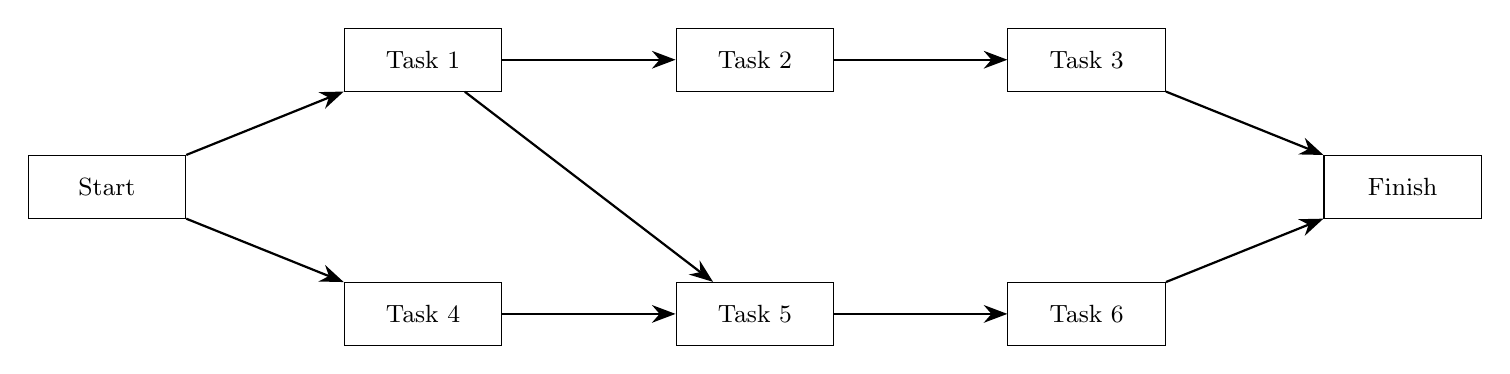
\begin{tikzpicture}[
  task/.style={rectangle, draw, minimum width=2cm, minimum height=0.8cm, font=\small},
  arr/.style={-{Stealth[length=3mm]}, thick},
  node distance=1.8cm and 2.2cm
]
  \node[task] (S) {Start};
  \node[task, above right=0.8cm and 2cm of S] (T1) {Task 1};
  \node[task, below right=0.8cm and 2cm of S] (T4) {Task 4};
  \node[task, right=of T1] (T2) {Task 2};
  \node[task, right=of T4] (T5) {Task 5};
  \node[task, right=of T2] (T3) {Task 3};
  \node[task, right=of T5] (T6) {Task 6};
  \node[task, below right=0.8cm and 2cm of T3] (F) {Finish};

  \draw[arr] (S) -- (T1);
  \draw[arr] (S) -- (T4);
  \draw[arr] (T1) -- (T2);
  \draw[arr] (T4) -- (T5);
  \draw[arr] (T2) -- (T3);
  \draw[arr] (T5) -- (T6);
  \draw[arr] (T3) -- (F);
  \draw[arr] (T6) -- (F);
  \draw[arr] (T1) -- (T5);
\end{tikzpicture}
\end{center}

% ── 2.2 Critical Path Method ────────────────────────────────
\subsection{Critical Path Method (CPM)}

\begin{definition}[Critical Path Method]
An algorithm that determines the \textbf{longest path} through a project network diagram, thereby determining the \textbf{minimum project duration}. Activities on this path have \textbf{zero float}.
\end{definition}

\begin{definition}[Key Dates for Each Activity]
Each activity is characterized by four dates:
\begin{itemize}[nosep]
  \item \textbf{Early Start (ES):} Earliest possible start date.
  \item \textbf{Early Finish (EF):} Earliest possible finish date.
  \item \textbf{Late Start (LS):} Latest start date without delaying the project.
  \item \textbf{Late Finish (LF):} Latest finish date without delaying the project.
\end{itemize}
\end{definition}

\begin{center}
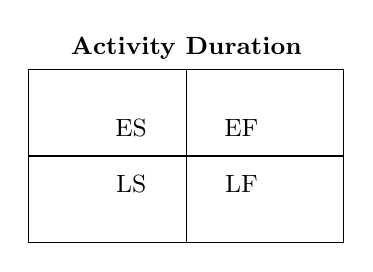
\begin{tikzpicture}
  \node[draw, minimum width=4cm, minimum height=2.2cm] (box) {};
  \node[above=0pt of box.north, font=\small\bfseries] {Activity Duration};
  \node[font=\small] at ([xshift=-0.7cm,yshift=0.35cm]box.center) {ES};
  \node[font=\small] at ([xshift=0.7cm,yshift=0.35cm]box.center) {EF};
  \node[font=\small] at ([xshift=-0.7cm,yshift=-0.35cm]box.center) {LS};
  \node[font=\small] at ([xshift=0.7cm,yshift=-0.35cm]box.center) {LF};
  \draw ([yshift=0cm]box.west) -- ([yshift=0cm]box.east);
  \draw ([xshift=0cm]box.north) -- ([xshift=0cm]box.south);
\end{tikzpicture}
\end{center}

\subsubsection{Forward Pass (Computing Early Dates)}

\begin{property}[Forward Pass Rules]
Starting from the \textbf{Start} node (set $\mathrm{ES} = \mathrm{EF} = 0$):
\begin{align}
  \mathrm{ES}_i &= \max\bigl(\mathrm{EF}_j \;\big|\; j \text{ is a predecessor of } i\bigr) \\
  \mathrm{EF}_i &= \mathrm{ES}_i + d_i
\end{align}
where $d_i$ is the duration of activity $i$.
\end{property}

\subsubsection{Backward Pass (Computing Late Dates)}

\begin{property}[Backward Pass Rules]
Starting from the \textbf{Finish} node (set $\mathrm{LS} = \mathrm{ES}$ of the Finish node):
\begin{align}
  \mathrm{LF}_i &= \min\bigl(\mathrm{LS}_j \;\big|\; j \text{ is a successor of } i\bigr) \\
  \mathrm{LS}_i &= \mathrm{LF}_i - d_i
\end{align}
\end{property}

\subsubsection{Float (Slack)}

\begin{definition}[Total Float]
The amount of time an activity can be delayed \textbf{without delaying the project end date}:
\[
  \text{Float}_i = \mathrm{LS}_i - \mathrm{ES}_i = \mathrm{LF}_i - \mathrm{EF}_i
\]
\begin{itemize}[nosep]
  \item Float $> 0$: schedule flexibility exists.
  \item Float $= 0$: the activity is \textbf{critical}.
\end{itemize}
\end{definition}

\begin{definition}[Free Float]
The amount of time an activity can be delayed \textbf{without delaying the early start of any successor activity}.
\end{definition}

\begin{definition}[Critical Path]
The sequence of activities with \textbf{float = 0}. It determines the overall project duration. Any delay on a critical-path activity delays the entire project.
\end{definition}

\begin{example}[Project Epsilon -- CPM Walkthrough]
Given the network with durations: Task~1 = 2, Task~2 = 4, Task~3 = 3, Task~4 = 7, Task~5 = 1, Task~6 = 5.

Dependencies: Start $\to$ T1, T4; T1 $\to$ T2, T5; T4 $\to$ T5; T2 $\to$ T3; T5 $\to$ T6; T3, T6 $\to$ Finish.

\medskip
\begin{tabular}{l c c c c c c}
\toprule
\textbf{Task} & \textbf{Duration} & \textbf{ES} & \textbf{EF} & \textbf{LS} & \textbf{LF} & \textbf{Float} \\
\midrule
Task 1 & 2 & 0 & 2 & 1 & 3  & 1 \\
Task 2 & 4 & 2 & 6 & 3 & 7  & 1 \\
Task 3 & 3 & 6 & 9 & 7 & 10 & 1 \\
Task 4 & 7 & 0 & 7 & 0 & 7  & 0 \\
Task 5 & 1 & 7 & 8 & 9 & 10 & 2 \\
Task 6 & 5 & 7 & 10 & 5 & 10 & \textbf{---} \\
\bottomrule
\end{tabular}

Note: Looking at the slides' values more carefully:
\begin{itemize}[nosep]
  \item T1: ES=0, EF=2, LS=1, LF=3, Float=1
  \item T2: ES=2, EF=6, LS=3, LF=7, Float=1
  \item T3: ES=6, EF=9, LS=7, LF=10, Float=1 (not on critical path in this configuration)
  \item T4: ES=0, EF=7, LS=0, LF=7, Float=\textbf{0} $\leftarrow$ Critical
  \item T5: ES=7, EF=8, LS=9, LF=10, Float=2
  \item T6: ES=5, EF=10, LS=5, LF=10, Float=\textbf{0} $\leftarrow$ Critical
\end{itemize}

\textbf{Critical Path:} Start $\to$ Task 4 $\to$ Task 6 $\to$ Finish. \textbf{Project Duration = 10 days.} (Note: the exact topology depends on additional links shown in slides; Task 6 connects after Task 2 finishes based on ES=5.)

From slide values: Float(T1)=1, Float(T2)=2, Float(T3)=5, Float(T4)=\textbf{0}, Float(T5)=1, Float(T6)=\textbf{0}. \\
\textbf{Critical Path:} Start $\to$ T4 $\to$ T6 $\to$ Finish (duration = $7 + 5 = 12$? No, project duration = 10 per slide). The critical path is derived by activities with float = 0.
\end{example}

\begin{remark}
The GANTT chart is the standard \textbf{schedule representation} derived from the CPM. It shows activities as horizontal bars plotted against time, making the schedule visually intuitive.
\end{remark}

% ── 2.3 Duration Compression ────────────────────────────────
\subsection{Duration Compression}

\begin{definition}[Duration Compression]
Techniques to shorten the project schedule \textbf{without changing the project scope}.
\end{definition}

\begin{definition}[Crashing]
Decreasing the duration of activities \textbf{on the critical path} by applying \textbf{additional resources}.
\begin{itemize}[nosep]
  \item Incurs \textbf{additional costs} due to lower efficiency.
  \item Strategy: crash activities that yield the \textbf{most time savings per dollar spent}.
  \item Source of \textbf{cost overrun}.
\end{itemize}
\end{definition}

\begin{definition}[Fast Tracking]
Performing normally \textbf{sequential} activities \textbf{in parallel} (or partially overlapping).
\begin{itemize}[nosep]
  \item Requires \textbf{redefining logical relationships} between activities.
  \item Often requires refining the WBS and Activity Lists.
  \item Considered \textbf{less costly} than crashing.
  \item Introduces \textbf{additional risks} due to potential rework (work starts before precise information from predecessors is available).
\end{itemize}
\end{definition}

\begin{example}
Starting coding before design is complete (fast tracking). Sending early code drops to the testing team before all code is finished.
\end{example}

\begin{warning}
Fast tracking increases risk of rework. Only apply it when schedule compression is critical and the risk is acceptable. Always document the rationale and associated risks.
\end{warning}

\begin{keytakeaways}
\begin{itemize}[nosep]
  \item CPM uses forward pass (ES, EF) and backward pass (LS, LF) to identify the critical path.
  \item \textbf{Float = LS $-$ ES = LF $-$ EF}; activities with float = 0 are critical.
  \item \textbf{Crashing} adds resources to critical-path activities $\Rightarrow$ higher cost.
  \item \textbf{Fast tracking} overlaps sequential tasks $\Rightarrow$ higher risk but lower cost than crashing.
  \item In Agile, the project-level schedule is less relevant; focus is on sprint schedules.
\end{itemize}
\end{keytakeaways}


%% ═══════════════════════════════════════════════════════════════
\section{Cost Budgeting and Baseline}
%% ═══════════════════════════════════════════════════════════════

\subsection{Cost Budgeting}

\begin{definition}[Cost Budgeting]
The process of merging \textbf{scope, cost, and schedule} information to establish a \textbf{cost baseline} against which project performance will be measured.
\end{definition}

\begin{definition}[Cost Baseline (S-Curve)]
A cumulative S-curve plotting \textbf{cumulative planned costs as a function of time}. Each point represents how much value is planned to be delivered at that moment.

\textbf{Cost accrual methods:}
\begin{itemize}[nosep]
  \item \textbf{Recommended:} Accrue 100\% of the cost when the task is planned to be \emph{completed}.
  \item \textbf{Alternative (50/50 rule):} Accrue 50\% when the task starts, remaining 50\% upon completion.
\end{itemize}
\end{definition}

\begin{definition}[BAC -- Budget At Completion]
The \textbf{total planned budget} for the project at time $t=0$. It is the final value on the cost baseline curve.
\[
  \mathrm{BAC} = \sum_{\text{all WP}} \text{Budgeted Cost of Work Package}
\]
\end{definition}

\begin{example}[Project Epsilon Cost Baseline]
With 1 person per task at \$1000/day:
\begin{itemize}[nosep]
  \item End of Task 4 (day 7): cumulative = \$7{,}000
  \item End of Task 1 (day 2): cumulative = \$2{,}000
  \item Progressive accumulation forms the S-curve
  \item BAC = \$22{,}000
\end{itemize}

The \% complete at any time $t$ is: $\frac{\text{Cost Baseline}(t)}{\text{BAC}} \times 100\%$.
\end{example}

\begin{remark}
Cost is treated as a proxy for \textbf{value delivered}: as each work package is completed, value is delivered to the project. This is a fundamental assumption in Earned Value Analysis.
\end{remark}

\subsection{Project Management Plan}

\begin{definition}[Project Management Plan]
The consolidation of \textbf{all planning outputs}: scope (WBS), cost estimates, schedules, cost baseline, communication plan, quality plan, risk management plan, and key decisions. It serves three purposes:
\begin{enumerate}[nosep, label=\arabic*.]
  \item Guide project execution.
  \item Facilitate communication among stakeholders.
  \item Provide a baseline for progress measurement and project control.
\end{enumerate}
\end{definition}

\begin{definition}[PMIS -- Project Management Information System]
Tools and techniques (manual and automated) used to gather, integrate, and disseminate the outputs of project management processes.
\end{definition}

\begin{keytakeaways}
\begin{itemize}[nosep]
  \item Cost budgeting merges scope + cost + schedule into the \textbf{cost baseline} (S-curve).
  \item BAC = total planned project cost = final point on the S-curve.
  \item The cost baseline is the \textbf{reference} for all performance measurement (EVA).
  \item The Project Management Plan consolidates all planning outputs into one reference document.
\end{itemize}
\end{keytakeaways}


%% ═══════════════════════════════════════════════════════════════
\section{Execution Management and Control}
%% ═══════════════════════════════════════════════════════════════

\subsection{Project Launching}

\begin{definition}[Project Execution]
The phase during which the product of the project is actually created. Work starts and charges to the project begin occurring.
\end{definition}

Key elements of launching:
\begin{itemize}[nosep]
  \item \textbf{Work Authorization System:} Formal procedure for sanctioning project work to ensure it is done at the right time and in proper sequence.
  \item \textbf{Project Kick-Off Meeting:} Builds team buy-in and morale.
  \item \textbf{Phase Gates:} Opportunities to celebrate completion or stop the project.
  \item \textbf{Resource Availability:} Anticipate and verify timely resource availability \emph{ahead of time}.
\end{itemize}

\subsection{Performance Reporting}

\begin{definition}[Performance Reporting]
The process of gathering, exchanging, and communicating information about project progress. Key activity: verifying what has been \textbf{actually completed} (at the work package level) with expected quality.
\end{definition}

Two channels of information:
\begin{enumerate}[nosep, label=\arabic*.]
  \item \textbf{Formal:} Structured periodic meetings (weekly, daily), reviews, status reports.
  \item \textbf{Informal:} Management by Wandering Around (MBWA), straight talk, alternative communication channels.
\end{enumerate}

\begin{remark}
Track items that are \textbf{not formally measured}: team morale, confidence, stress levels. These are often leading indicators of future problems.
\end{remark}

\subsection{Earned Value Analysis (EVA)}

\begin{definition}[Earned Value Analysis]
A technique that \textbf{integrates scope, cost, and schedule} to assess project performance by comparing three key values at any point in time:
\begin{enumerate}[nosep, label=\arabic*.]
  \item \textbf{BCWS} (Budgeted Cost of Work Scheduled) = \textbf{Planned Value (PV)}: budget to date --- ``what we should have delivered.''
  \item \textbf{BCWP} (Budgeted Cost of Work Performed) = \textbf{Earned Value (EV)}: budget of work actually completed --- ``what we have actually delivered.''
  \item \textbf{ACWP} (Actual Cost of Work Performed) = \textbf{Actual Cost (AC)}: total costs actually incurred --- ``what we have actually spent.''
\end{enumerate}
\end{definition}

\begin{definition}[Estimating BCWP]
Two methods:
\begin{itemize}[nosep]
  \item \textbf{0/100 Rule (Recommended):} Accrue 100\% of budgeted cost only when a task is \emph{complete}; 0\% otherwise.
  \item \textbf{50/50 Rule:} Accrue 50\% when a task starts, remaining 50\% upon completion. Provides a statistical approximation when many tasks are considered but \textbf{bears higher risks}. Not recommended.
\end{itemize}
\end{definition}

\subsubsection{Variance Indicators}

\begin{formulabox}[EVA Variance Formulas]
\textbf{Schedule Variance:}
\[
  \mathrm{SV} = \mathrm{BCWP} - \mathrm{BCWS}
\]
\begin{itemize}[nosep]
  \item $\mathrm{SV} < 0$: schedule \textbf{delay}
  \item $\mathrm{SV} > 0$: \textbf{ahead} of schedule
\end{itemize}

\textbf{Cost Variance:}
\[
  \mathrm{CV} = \mathrm{BCWP} - \mathrm{ACWP}
\]
\begin{itemize}[nosep]
  \item $\mathrm{CV} < 0$: cost \textbf{overrun}
  \item $\mathrm{CV} > 0$: cost \textbf{under run} (saving money)
\end{itemize}
\end{formulabox}

\subsubsection{Performance Indices}

\begin{formulabox}[EVA Performance Indices]
\textbf{Schedule Performance Index:}
\[
  \mathrm{SPI} = \frac{\mathrm{BCWP}}{\mathrm{BCWS}}
\]
\begin{itemize}[nosep]
  \item $\mathrm{SPI} < 1$: schedule delay
  \item $\mathrm{SPI} > 1$: ahead of schedule
\end{itemize}

\textbf{Cost Performance Index:}
\[
  \mathrm{CPI} = \frac{\mathrm{BCWP}}{\mathrm{ACWP}}
\]
\begin{itemize}[nosep]
  \item $\mathrm{CPI} < 1$: cost overrun
  \item $\mathrm{CPI} > 1$: cost under run
\end{itemize}
\end{formulabox}

\subsubsection{Estimate At Completion (EAC)}

\begin{definition}[EAC -- Estimate At Completion]
A forecast of total project costs based on current performance. Three scenarios:
\end{definition}

\begin{formulabox}[EAC Formulas]
\textbf{Scenario 1 -- Variance is typical} (expected to continue):
\[
  \mathrm{EAC} = \frac{\mathrm{BAC}}{\mathrm{CPI}}
\]
CPI is shown to be relatively stable after 15--20\% project completion.

\textbf{Scenario 2 -- Variance was exceptional} (will not recur):
\[
  \mathrm{EAC} = \mathrm{ACWP}_{\text{to date}} + \text{Remaining Budget}
\]

\textbf{Scenario 3 -- Assumptions changed} (new estimate required):
\[
  \mathrm{EAC} = \mathrm{ACWP}_{\text{to date}} + \text{New Estimate for Remaining Work}
\]
\end{formulabox}

\begin{example}[Project Epsilon EVA]
On March 18 (end of day), with Tasks 1, 2, 4, and 6 completed. ACWP = \$19{,}000.

From the cost baseline (S-curve), the BCWS at that date corresponds to the planned cumulative value.

BCWP = budgeted costs of completed tasks:
\[
  \mathrm{BCWP} = 2000 + 4000 + 7000 + 5000 = \$18{,}000
\]
\begin{itemize}[nosep]
  \item $\mathrm{CV} = 18{,}000 - 19{,}000 = -\$1{,}000$ $\Rightarrow$ cost overrun
  \item $\mathrm{CPI} = 18{,}000 / 19{,}000 \approx 0.947$ $\Rightarrow$ for every dollar spent, only \$0.95 of value delivered
  \item $\mathrm{EAC} = 22{,}000 / 0.947 \approx \$23{,}232$ (if variance is typical)
\end{itemize}
\end{example}

\begin{remark}
In Agile, without a traditional project schedule and cost budgeting, Earned Value Analysis is \textbf{not directly applicable}. Agile uses velocity and burndown charts instead.
\end{remark}

\subsection{Cost and Schedule Control}

\begin{definition}[Cost/Schedule Control]
The processes of:
\begin{itemize}[nosep]
  \item Analyzing causes of cost/schedule variances.
  \item Deciding if corrective action is needed.
  \item Updating cost estimates (EAC) and project schedule.
  \item Managing changes, actions, and updates.
\end{itemize}
When justified, the Project Management Plan may be \textbf{re-baselined} with new estimates.
\end{definition}

\subsection{Anticipation Best Practices}

Key anticipation strategies:
\begin{itemize}[nosep]
  \item Thorough \textbf{risk management} and detecting \textbf{symptoms} early.
  \item Secure commitments with periodical checking.
  \item Carefully manage \textbf{prerequisites}.
  \item Avoid \textbf{black boxes} (no visibility for long periods).
  \item Immediately focus on \textbf{small delays} --- do not wait.
  \item Stay at least \textbf{one move ahead} on the critical path.
\end{itemize}

\subsection{Change Management}

\begin{definition}[Change Management]
A formal process to handle changes to project scope, schedule, or cost:
\begin{enumerate}[nosep, label=\arabic*.]
  \item \textbf{Formal Request:} Document the proposed change.
  \item \textbf{Impact Analysis:} Assess effects on cost, schedule, risks, quality.
  \item \textbf{Decision:} Approve/reject via a Change Review Board.
  \item \textbf{Update:} Revise the Project Management Plan accordingly.
\end{enumerate}
\end{definition}

\begin{remark}
In Agile, change management is embedded in the process (backlog refinement). However, ensure that \textbf{fixed scope is not contracted} --- i.e., the contracted scope should not be unilaterally changed.
\end{remark}

\begin{keytakeaways}
\begin{itemize}[nosep]
  \item EVA compares three values: BCWS (planned), BCWP (earned), ACWP (actual).
  \item $\mathrm{SV} = \mathrm{BCWP} - \mathrm{BCWS}$; $\mathrm{CV} = \mathrm{BCWP} - \mathrm{ACWP}$.
  \item $\mathrm{SPI} = \mathrm{BCWP}/\mathrm{BCWS}$; $\mathrm{CPI} = \mathrm{BCWP}/\mathrm{ACWP}$.
  \item $\mathrm{EAC} = \mathrm{BAC}/\mathrm{CPI}$ if variance is typical.
  \item Change management: formal request $\to$ impact analysis $\to$ decision $\to$ update.
  \item Anticipate: detect symptoms, avoid black boxes, address small delays immediately.
\end{itemize}
\end{keytakeaways}


%% ═══════════════════════════════════════════════════════════════
\section{Risk Management}
%% ═══════════════════════════════════════════════════════════════

\subsection{Enterprise vs.\ Project Risk Management}

\begin{definition}[Enterprise Risk Management (ERM)]
A comprehensive framework (ISO 31000) covering:
\begin{itemize}[nosep]
  \item \textbf{Operational Risks} (business management)
  \item \textbf{Financial Risks} (investment management)
  \item \textbf{Strategic Risks} (enterprise change management)
  \item \textbf{Hazard Risks} (casualty/actuarial)
\end{itemize}
Project Risk Management is a \textbf{subset} of ERM, focused on risks within a specific project.
\end{definition}

\subsection{The Notion of Risk}

\begin{definition}[Risk (Project Management)]
An \textbf{uncertain event} whose outcome could affect the project. Unlike the general language definition (always negative), PM risks are of two kinds:
\begin{itemize}[nosep]
  \item \textbf{Opportunities:} Positive outcomes.
  \item \textbf{Threats:} Negative outcomes.
\end{itemize}
\end{definition}

\begin{definition}[Purpose of Risk Management]
Anticipate uncertain events to ensure the project meets its targets:
\begin{itemize}[nosep]
  \item Prevent surprises (especially bad ones) --- avoid management by crisis.
  \item Prevent problems from occurring or minimize their impact.
  \item Recognize opportunities before competitors.
  \item Maximize results of positive events, minimize consequences of adverse events.
\end{itemize}
\end{definition}

\subsection{Risk Management Process}

The risk management process consists of five steps:

\begin{enumerate}[label=\textbf{\arabic*.}]
  \item \textbf{Risk Management Planning}
  \item \textbf{Risk Identification}
  \item \textbf{Risk Analysis} (Qualitative and Quantitative)
  \item \textbf{Risk Response Planning}
  \item \textbf{Risk Monitoring and Control}
\end{enumerate}

\subsubsection{Risk Identification}

\begin{definition}[Risk Identification]
Determining which risks are likely to affect the project and documenting their characteristics. Identify the main \textbf{sources of risk} and possible \textbf{risk events}.
\end{definition}

\textbf{Two major initial sources of risks in projects:}
\begin{enumerate}[nosep, label=\arabic*.]
  \item \textbf{SCOPE (WBS):} The WBS identifies all deliverables; failure to produce any deliverable is a risk.
  \item \textbf{RESOURCES:} Unavailability of resources according to the project schedule.
\end{enumerate}

\textbf{Technique:} Brainstorming (creativity is needed).

\subsubsection{Risk Analysis}

\begin{definition}[Risk Analysis Parameters]
For each identified risk event, estimate:
\begin{itemize}[nosep]
  \item \textbf{Probability of occurrence} ($P$): may use historical data, company statistics.
  \item \textbf{Impact / Range of outcomes} ($I$): cost of the work package at risk, contract penalties, lost revenue, or qualitative rating.
  \item \textbf{Expected timing and frequency.}
  \item \textbf{Detection indicators (risk symptoms):} indirect manifestations (e.g., cost overruns may indicate poor estimating; low morale may indicate difficulties).
\end{itemize}
\end{definition}

\begin{formulabox}[Expected Monetary Value (EMV)]
\[
  \mathrm{EMV} = P \times I
\]
where $P$ = probability of the risk event and $I$ = monetary impact (value).

EMVs can be aggregated to calculate a \textbf{range of total project costs} or define \textbf{contingencies}.
\end{formulabox}

\begin{definition}[Risk Classification for Response]
From the list of identified risk events, classify each as:
\begin{itemize}[nosep]
  \item \textbf{Opportunities to pursue} (warrant response)
  \item \textbf{Opportunities to ignore}
  \item \textbf{Threats to respond to} (warrant response)
  \item \textbf{Threats to accept}
\end{itemize}
For ignored opportunities and accepted threats: \textbf{document the decision and who made it}.
\end{definition}

\begin{example}[Risk Priority Matrix]
~\\
\begin{tabular}{l c c c}
\toprule
\textbf{Risk Event} & \textbf{Probability} & \textbf{Impact} & \textbf{Respond?} \\
\midrule
Risk Event 1 & High   & High   & Yes \\
Risk Event 2 & High   & Medium & Yes \\
Risk Event 3 & Medium & High   & Yes \\
Risk Event 4 & Medium & Medium & Yes \\
Risk Event 5 & Medium & Low    & No  \\
Risk Event 6 & Low    & Medium & No  \\
Risk Event 7 & Low    & Low    & No  \\
\bottomrule
\end{tabular}
\end{example}

\subsubsection{Risk Response Planning}

\begin{definition}[Risk Response Strategies for Threats]
Three categories:
\begin{enumerate}[nosep, label=\arabic*.]
  \item \textbf{Avoidance:} Eliminate the threat by changing the project plan (e.g., change the WBS, adopt a safer design approach).
  \item \textbf{Mitigation:} Reduce the \textbf{probability} or \textbf{impact} of the risk event (e.g., plan contingencies, add safety margins).
  \item \textbf{Acceptance:} Acknowledge the risk and take no proactive action; deal with it if it occurs.
\end{enumerate}
\end{definition}

\begin{example}[Electronic Card Design]
\textbf{Risk:} One-pass design for electronic cards bears high risk of rework if a bug is found late.
\begin{itemize}[nosep]
  \item \textbf{Avoidance:} Switch to a two-pass design (longer but safer). Impacts: larger scope, longer schedule, higher cost, better quality.
  \item \textbf{Mitigation:} Keep one-pass design but plan physical layout with external connection points for quick fixes. More costly but saves time vs.\ two-pass.
  \item \textbf{Acceptance:} Keep one-pass design to meet customer deadlines; assign best engineers.
\end{itemize}
\end{example}

\begin{example}[Car Travel Risk]
Source of risk: travelling by car to work.\\
Risk event: accident.
\begin{itemize}[nosep]
  \item \textbf{Avoidance:} Walk to work, take public transport, or work from home.
  \item \textbf{Mitigation:} Insurance, advanced driving lessons, buy a safe car, always fasten seatbelt.
  \item \textbf{Acceptance:} No specific action.
\end{itemize}
\end{example}

\begin{definition}[Risk Response Planning Output]
Two types of planned actions:
\begin{enumerate}[nosep, label=\arabic*.]
  \item \textbf{Immediate actions:} Integrated into the WBS and Project Management Plan (preventive measures).
  \item \textbf{Contingency actions:} Executed only if and when the risk event occurs.
\end{enumerate}
The \textbf{Risk Management Plan} documents: procedures, risk identification/analysis results, responsibilities, and responses developed.
\end{definition}

\subsubsection{Risk Monitoring and Control}

\begin{definition}[Risk Monitoring and Control]
The process of:
\begin{itemize}[nosep]
  \item Detecting risk occurrence.
  \item Executing planned risk responses.
  \item Analyzing changes in risk over the project lifecycle.
  \item Repeating the identify $\to$ analyze $\to$ respond cycle when changes occur.
\end{itemize}
\end{definition}

\begin{definition}[Workaround]
An \textbf{unplanned response} to a negative risk event that was not anticipated in the risk management plan.
\end{definition}

\textbf{When an unplanned event occurs:}
\begin{itemize}[nosep]
  \item Avoid panic; avoid blame.
  \item Look for creativity: brainstorming, out-of-the-box thinking.
  \item Get help from management or the client as needed.
\end{itemize}

\begin{keytakeaways}
\begin{itemize}[nosep]
  \item Risks = \textbf{opportunities} (positive) + \textbf{threats} (negative).
  \item Risk process: Plan $\to$ Identify $\to$ Analyze $\to$ Respond $\to$ Monitor \& Control.
  \item Two major risk sources in projects: \textbf{Scope (WBS)} and \textbf{Resources}.
  \item $\mathrm{EMV} = P \times I$ for quantitative risk assessment.
  \item Three response strategies for threats: \textbf{Avoidance, Mitigation, Acceptance}.
  \item A \textbf{workaround} is an unplanned response to an unanticipated risk.
  \item Always document accepted risks and who made the decision.
\end{itemize}
\end{keytakeaways}


%% ═══════════════════════════════════════════════════════════════
\section{Quality Management}
%% ═══════════════════════════════════════════════════════════════

\subsection{Why Quality?}

Quality is a \textbf{business matter}:
\begin{enumerate}[nosep, label=\arabic*.]
  \item \textbf{Win \& Keep Clients:} Meet client expectations; quality certifications as a marketing weapon.
  \item \textbf{Optimize Costs to Optimize Profit:} Total Cost of Quality; defect \emph{prevention} vs.\ defect \emph{correction}.
\end{enumerate}

\begin{definition}[Quality (ISO 9000)]
The ability of a product, system, or process (set of characteristics) to satisfy \textbf{customer and other stakeholders' requirements}.
\[
  \text{Quality} = \text{Satisfying Client Needs at the Best Cost}
\]
\end{definition}

\subsection{Two Approaches to Quality}

\begin{definition}[Quality Assurance (QA)]
\textbf{Short-term} approach pursuing conformance to specifications and satisfying customer needs. A set of \textbf{predefined actions} providing confidence that a product/service will satisfy requirements.
\end{definition}

\begin{definition}[Continuous Improvement]
\textbf{Long-term} approach based on improving the application area process. Pursues \textbf{excellence} and \textbf{value attributes}.
\end{definition}

\subsection{Planning for Quality}

The Quality Plan includes:
\begin{enumerate}[nosep, label=\arabic*.]
  \item Methods used.
  \item QA reviews performed (result in actions $\to$ WBS items $\to$ scope).
  \item Continuous improvement by injecting lessons learned.
  \item Mindset through education.
\end{enumerate}

\subsection{The Four Quality Types}

\begin{definition}[Quality vs.\ Grade]
Quality is often opposed to Grade. \textbf{Low quality is always a problem; low grade may not be.} Zero defect $\neq$ value.
\end{definition}

\subsubsection{1. Conformance to Specifications (Provider Logic)}

\begin{itemize}[nosep]
  \item Development of standards (public and customer specifications).
  \item Conformance must be \textbf{verified} through quality control.
  \item Examples: interoperability tests, homologation tests.
  \item Reliability is an important criterion for \textbf{sustainability}.
\end{itemize}

\subsubsection{2. Excellence (Provider Logic)}

\begin{itemize}[nosep]
  \item Quest for perfection (zero defect, Six Sigma).
  \item Originated from craftsmanship; quality problems appeared with industry/volume production.
  \item Think of \textbf{economical constraints}: no gold plating.
  \item Reduce the \textbf{Total Cost of Quality}: prevention vs.\ correction.
\end{itemize}

\begin{warning}
\textbf{No Gold Plating:} Do not add features or quality beyond what was specified. Use Value Analysis to determine what is worth investing in.
\end{warning}

\subsubsection{3. Satisfying Customer Expectations (Customer Logic)}

\begin{itemize}[nosep]
  \item Most common quality definition today (driven by the growth of the services market).
  \item Some expectations are hard to capture in written specifications.
  \item Strategies: maximize formal capture, think of \textbf{implied} (not explicit) expectations, periodically verify with client (prototypes, etc.).
\end{itemize}

\subsubsection{4. Value Attribute (Customer Logic)}

\begin{definition}[Value Attribute]
Quality viewed through the \textbf{price/quality ratio}: what the customer gets for what they pay.
\end{definition}

\begin{definition}[Value Analysis / Value Engineering]
A product is seen as a \textbf{set of functions} (vs.\ a set of components). Process:
\begin{enumerate}[nosep, label=\arabic*.]
  \item \textbf{Functional Analysis:} Understand client needs (explicit and implicit), understand competition.
  \item For each function, estimate \textbf{client value} and \textbf{cost}.
  \item \textbf{Prioritize} to establish functional specifications.
\end{enumerate}
\end{definition}

\begin{definition}[Value Management / Customer Value Management]
A complete business management system that:
\begin{itemize}[nosep]
  \item Understands customer purchase and repurchase behaviors.
  \item Adapts products and processes accordingly.
\end{itemize}
\end{definition}

\subsection{Quality Logics Summary}

\begin{center}
\begin{tabular}{l c c}
\toprule
& \textbf{Customer Logic} & \textbf{Provider Logic} \\
\midrule
\textbf{QA (Short Term)} & Satisfying Customer Needs & Conformance to Specifications \\
\textbf{CI (Long Term)}  & Value Attributes & Excellence \\
\bottomrule
\end{tabular}
\end{center}

\subsection{Main Tools for Quality}

\begin{definition}[Quality Assurance Reviews]
\textbf{Independent} review activities performed by specially trained, authorized individuals. QA reviews include:
\begin{itemize}[nosep]
  \item Ensuring high-quality, profitable solutions.
  \item Recognition, containment, and mitigation of risks.
  \item Sustainability reviews may also be included.
\end{itemize}
\end{definition}

\begin{definition}[Continuous Process Improvement]
\begin{enumerate}[nosep, label=\arabic*.]
  \item Document formal processes.
  \item Continuously examine performance.
  \item Update business processes to: proliferate best practices, correct defects.
\end{enumerate}
\end{definition}

\subsection{Quality Hints (Best Practices)}

\begin{itemize}[nosep]
  \item Think of quality \textbf{from the customer's point of view}.
  \item Turn implied needs into stated needs through \textbf{scope management}.
  \item Prioritize functions to deliver \textbf{value}.
  \item Quality $\neq$ Grade: low quality is always a problem.
  \item Zero defect does NOT mean you have value.
  \item Project Quality Management addresses both the \textbf{quality of the project} and the \textbf{product of the project}.
  \item Use \textbf{independent reviews}.
  \item Continuously improve by learning (\textbf{Lessons Learned}).
\end{itemize}

\begin{remark}
Quality Assurance often performs Risk Management. The purpose of QA reviews includes recognition, containment, and mitigation of risks that could jeopardize project success.
\end{remark}

\begin{keytakeaways}
\begin{itemize}[nosep]
  \item Four quality types: Conformance to Specs, Excellence, Customer Expectations, Value Attribute.
  \item Quality $\neq$ Grade; low quality is always a problem.
  \item Two logics: Customer (expectations, value) vs.\ Provider (specs, excellence).
  \item Two approaches: QA (short-term) vs.\ Continuous Improvement (long-term).
  \item Value Analysis: view product as functions, prioritize by client value/cost ratio.
  \item QA reviews must be \textbf{independent} and may include risk and sustainability assessments.
\end{itemize}
\end{keytakeaways}


%% ═══════════════════════════════════════════════════════════════
\section{Project Closing and Conclusion}
%% ═══════════════════════════════════════════════════════════════

\subsection{Closing the Project}

\begin{definition}[Project Closure]
Every project requires formal closure, which involves:
\begin{itemize}[nosep]
  \item \textbf{Administrative closure} + \textbf{Contract close-out} (procurement).
  \item Verifying and documenting project results.
  \item \textbf{Formal acceptance:} Documentation that the client/sponsor has accepted the product.
  \item Documenting \textbf{Lessons Learned} for continuous improvement.
\end{itemize}
\end{definition}

\begin{definition}[Administrative Closure Checklist]
\begin{itemize}[nosep]
  \item All invoicing has been issued.
  \item No pending change requests (any pending must be reviewed).
  \item All project-related costs have been claimed/transferred to contract:
  \begin{itemize}[nosep]
    \item Labor costs
    \item Travel costs
    \item Asset-related costs
    \item Subcontractor-related costs
  \end{itemize}
\end{itemize}
\end{definition}

\subsection{Communication and Management Tips}

Best practices for project managers:
\begin{itemize}[nosep]
  \item Set priorities and address high-priority items first.
  \item Manage stakeholders' expectations actively.
  \item Meeting minutes: set baseline, document decisions, assign actions.
  \item Write key agreements formally.
  \item Plan for communication explicitly.
  \item Manage stress and workload.
  \item \textbf{Fast start:} the schedule battle is often lost in the early days.
  \item Thorough planning and thorough change management.
  \item Verify status through \textbf{both formal and informal} channels.
\end{itemize}

\subsection{Root Causes of Troubled Projects}

\begin{definition}[Root Causes -- Design/Proposal Phase]
\begin{itemize}[nosep]
  \item Inaccurate project estimates.
  \item Failure to set and manage customer expectations.
  \item Overlooking stakeholders' expectations management.
  \item Failure to establish an appropriate contractual baseline.
  \item Failure to reach a common understanding of requirements or completion criteria.
  \item Failure to plan for risk containment.
  \item Concessions during negotiations with no price adjustment.
\end{itemize}
\end{definition}

\begin{definition}[Root Causes -- Delivery Phase]
\begin{itemize}[nosep]
  \item Lack of or inadequate project management discipline.
  \item Ineffective financial management.
  \item Failure to implement a proper change management process.
  \item Lack of or inadequate project management plan/schedule.
  \item Inability to acquire properly skilled resources.
  \item Unfulfilled customer responsibilities.
  \item Overlooking stakeholders' expectations management.
\end{itemize}
\end{definition}

\begin{keytakeaways}
\begin{itemize}[nosep]
  \item Every project needs formal \textbf{administrative closure} and \textbf{formal acceptance}.
  \item Document \textbf{Lessons Learned} systematically for organizational learning.
  \item Most troubled projects fail due to: poor estimates, unmanaged expectations, inadequate change management, and insufficient planning discipline.
  \item The schedule battle is often lost in the \textbf{early days} --- fast start is critical.
  \item Verify status through \textbf{both formal and informal channels}.
\end{itemize}
\end{keytakeaways}

\end{document}
